\chapter{Tournament Results}

In this chapter, I will show how the agents described in the previous sections perform using different configurations in tournament experiments. 
To ensure fairness when comparing AI agents, each agent needs to have the same amount of resources. When comparing AI agents
in computer games in general, this is usually achieved by setting a time limit for average move time. Especially for Sagrada,
counting on that each game consists of 20 turns, I decided to set this time limit to 300ms. 

All the experiments present in this section were run on a computer with Ubuntu distribution. It has an AMD Ryzen 7 5800H CPU with 8 cores and 16 threads and 16GB of RAM. 
I am using an optimized build of the tournament executable that is achieved by adding the \texttt{--buildtype=debugoptimized} flag to the Meson build command.

\section{MCTS}

The MCTS agent has 4 configurable parameters that are grouped in \texttt{the MCTSPlayerContext structure} described in the introduction part 
of the Chapter \ref{chap:MCTS} . In this section, I will try to find the strongest possible configurations through experiments against different agents. 

\subsection{Playout Strategies}

Choosing the strongest playout strategy is about finding the perfect balance between speed and strength. In this section, I will talk about
the results of 4 different playout strategies. These are other AI agents that can play games on their own. Namely, these are the First agent,
both strategies of the Rules-based agent and the Minimax agent with a search depth of 1.

First, I am finding the number of iterations for each playout strategy that fits the time limit by manually experimenting until the desired results are achieved.
The following table displays the results of these experiments:

\begin{table}[H] 
    \centering
    \begin{tabular}{c|c} 
        \textbf{Playout strategy} & \textbf{Iteration count} \\ \hline
        First & 5400 \\ \hline
        Minimax & 230 \\ \hline
        Rules-based only dtfm & 820 \\ \hline
        Rules-based all moves & 300 \\ 
    \end{tabular}
    \caption{Iteration count that fits the time limit for the chosen playout strategies}
    %\label{tab:example_table}
\end{table}

\subsection{Determinizing World Count and Exploration Constant}

According to the results from the previous section, the different playout strategies have varying usable iterations to fit the time limit capacity.
This means that dividing the total number of iterations in the determinizing worlds and choosing a strong matching exploration constant is expected to be
different for the playout agents.

The branching factor plays an important role in this algorithm because according to the selection phase described in Section \ref{sec:MCTS_Selection},
the first N iterations of the algorithm simply explore all the possible moves from the current state. This means that if the iteration count is set too low, the exploration 
constant is negligible. For this reason, I ran an experiment to get the average branching factor for the 4 playout strategies each run in 100 games against the Minimax agent.
The following figure illustrates the results:

\begin{figure}[H]
    \caption{Average branching factor for the MCTS agent's all playout strategies}
    \centerline{\mbox{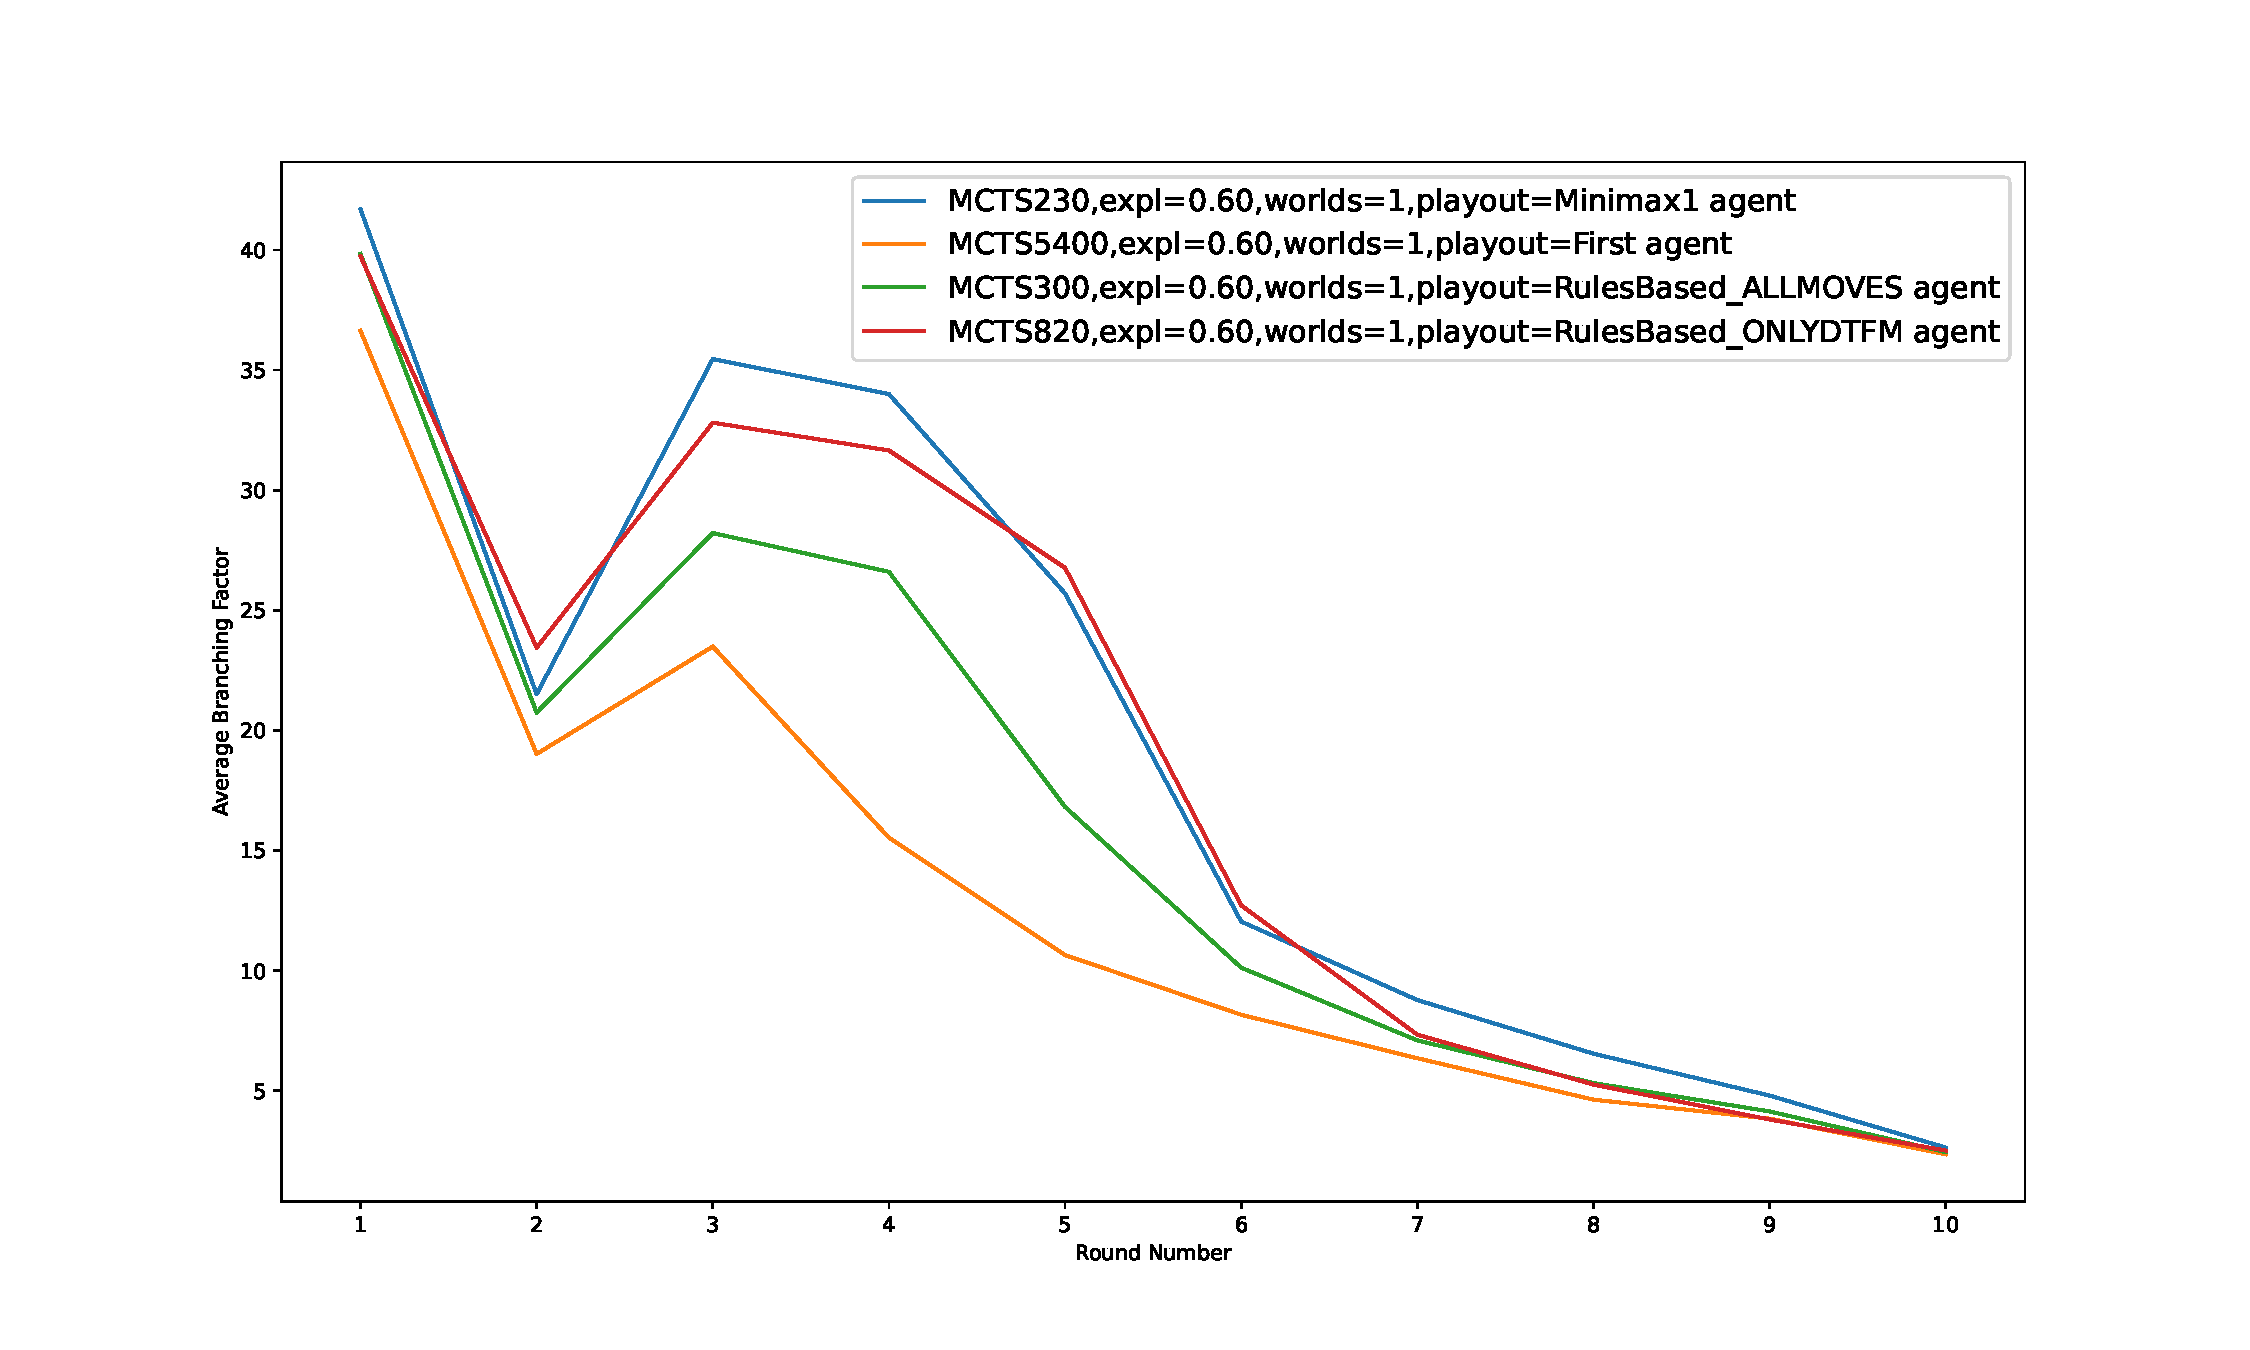
\includegraphics[width=180mm]{img/mcts_average_branching_factor.pdf}}}
    \label{fig:example}
\end{figure}

The figure shows that the average branching factor for the MCTS agents is the highest in round 1 with a value slightly above 40. So the algorithm's selection
strategy could make a higher difference, I choose to configure a minimum of 80 iteration count for the agents. 


As already mentioned in Section \ref{subsec:MCTS_Selection_UCT}, an often chosen value for the exploration constant is $\sqrt{2}$. I chose to experiment with 
values $[0.6, 0.8, 1.0, 1.2, 1.4, 1.6, 1.8, 2.0]$. I ran separate experiments for the four playout strategies. The following figures illustrate the highest
win count in every iteration count-determinizing world count division displaying the exploration constant used. Each tournament contained 100 games and every
exploration constant, iteration count-determinizing world count pair has a corresponding tournament. The results can be found in the \texttt{tournament\_results/mcts\_playout\_first\_exploration},
\texttt{tournament\_results/mcts\_playout\_minimax1\_exploration}, \\ \texttt{tournament\_results/mcts\_playout\_rules\_based\_only\_dtfm\_exploration} and the 
\texttt{tournament\_results/mcts\_playout\_rules\_based\_all\_moves\_exploration} directories. All the tournaments were run against the Minimax agent with search depth of 3
and determinizing world count of 1.

\begin{figure}[H]
    \caption{Exploration constants producing the highest win rate in different iteration count-determinizing world count divisions for the First playout}
    \centerline{\mbox{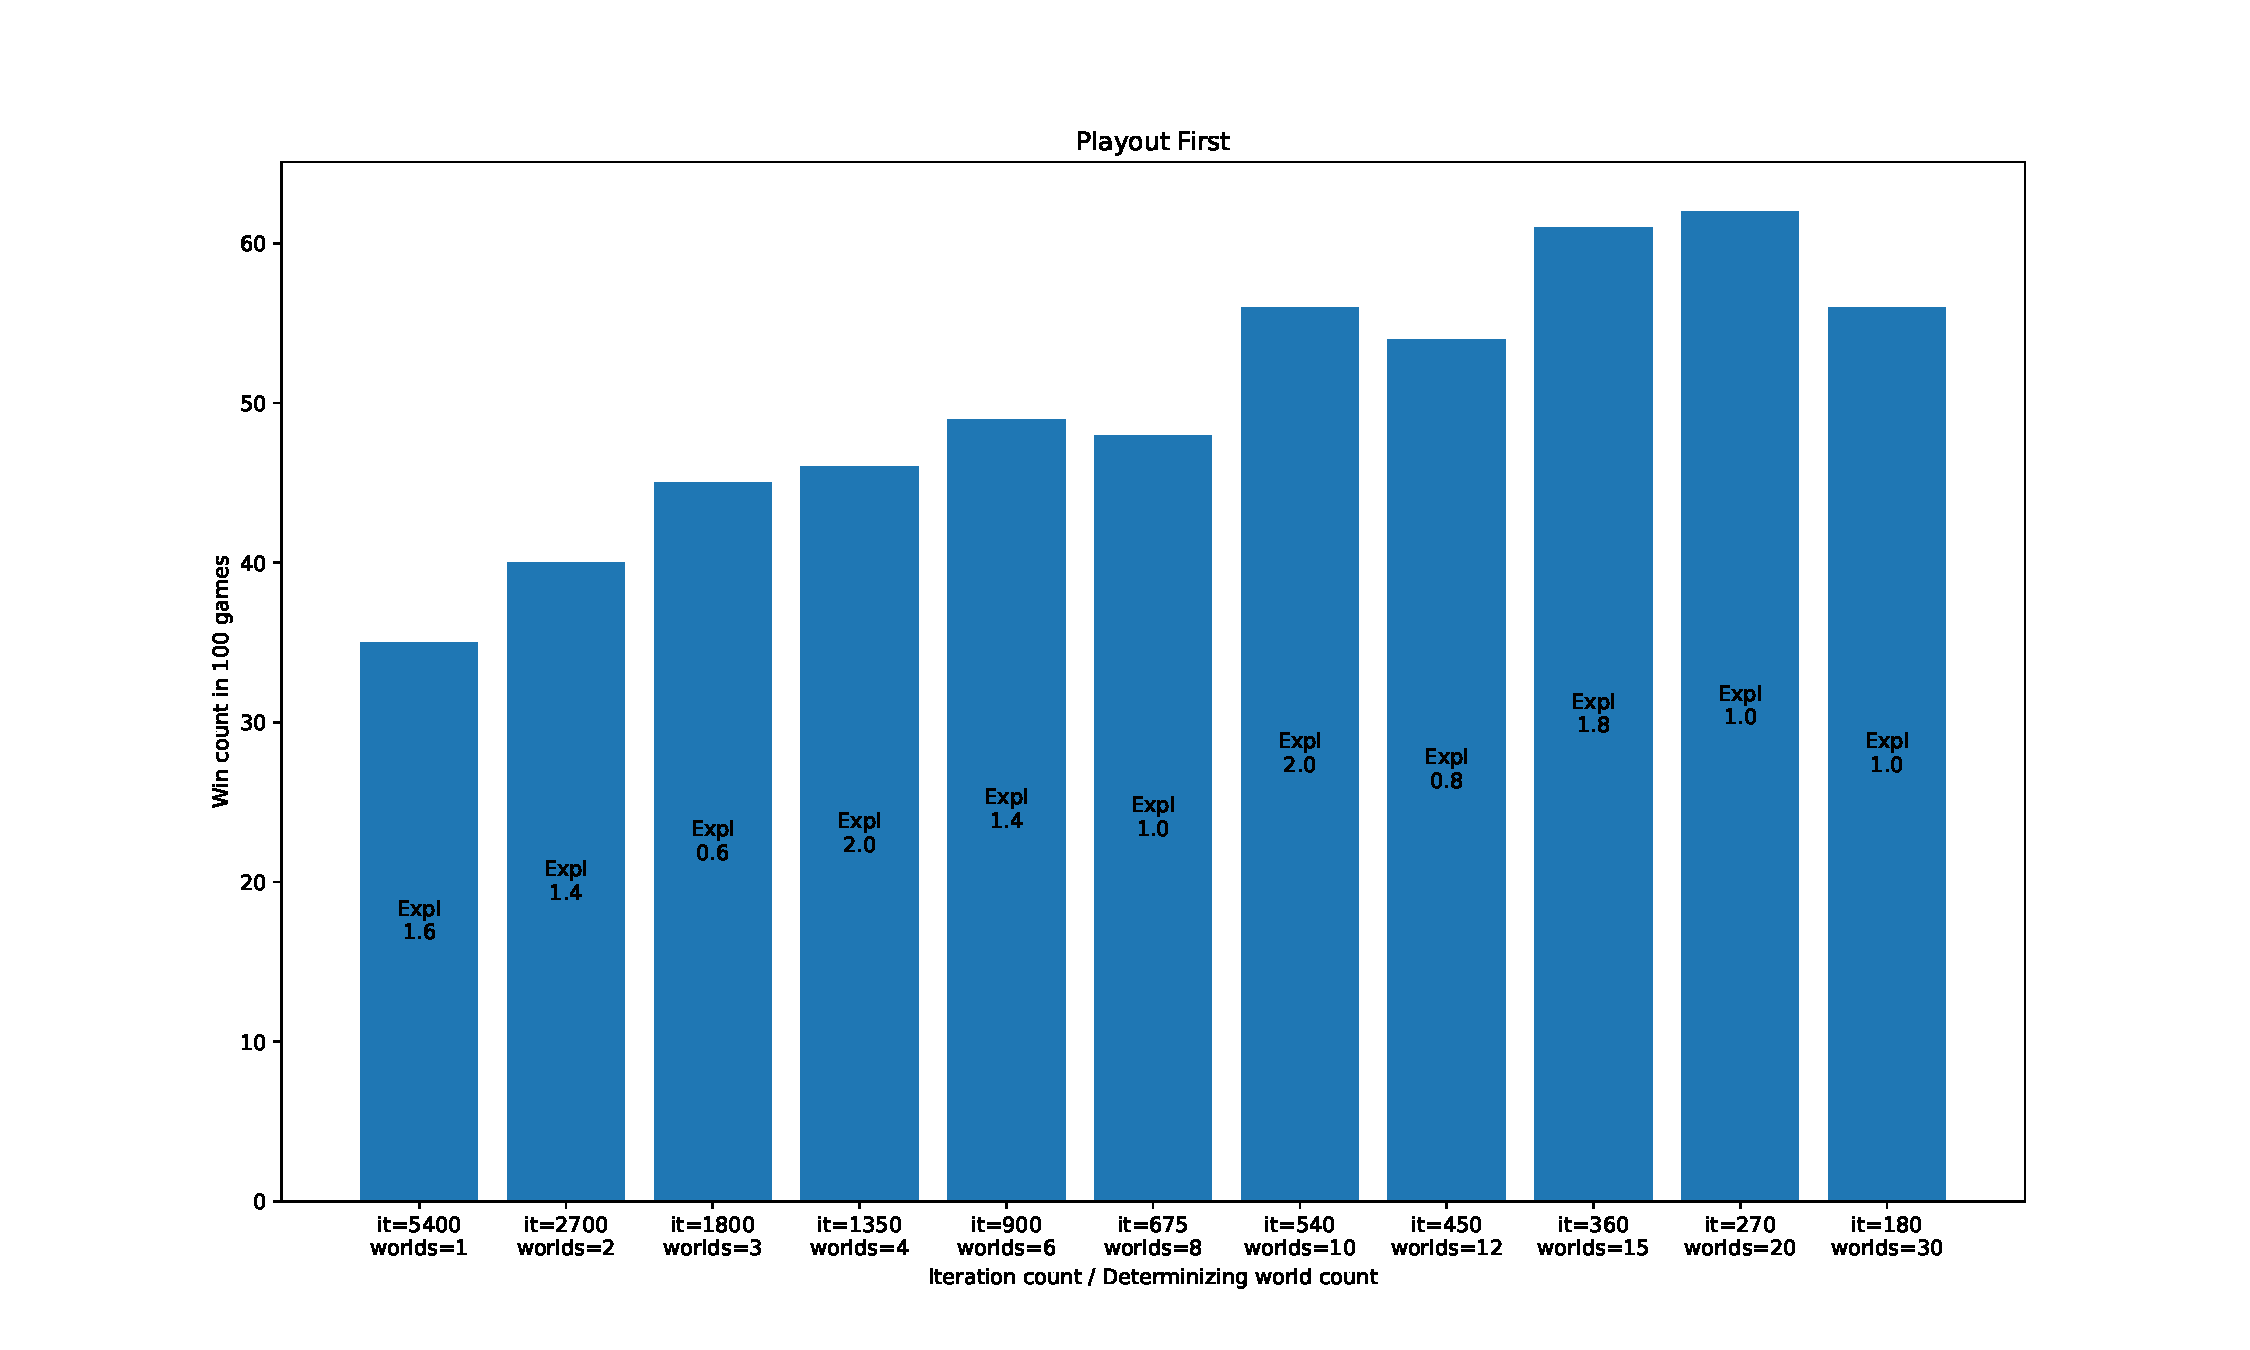
\includegraphics[width=180mm]{img/mcts_expl_worldcount_First.pdf}}}
    \label{fig:example}
\end{figure}

\begin{figure}[H]
    \caption{Exploration constants producing the highest win rate in different iteration count-determinizing world count divisions for the Minimax playout}
    \centerline{\mbox{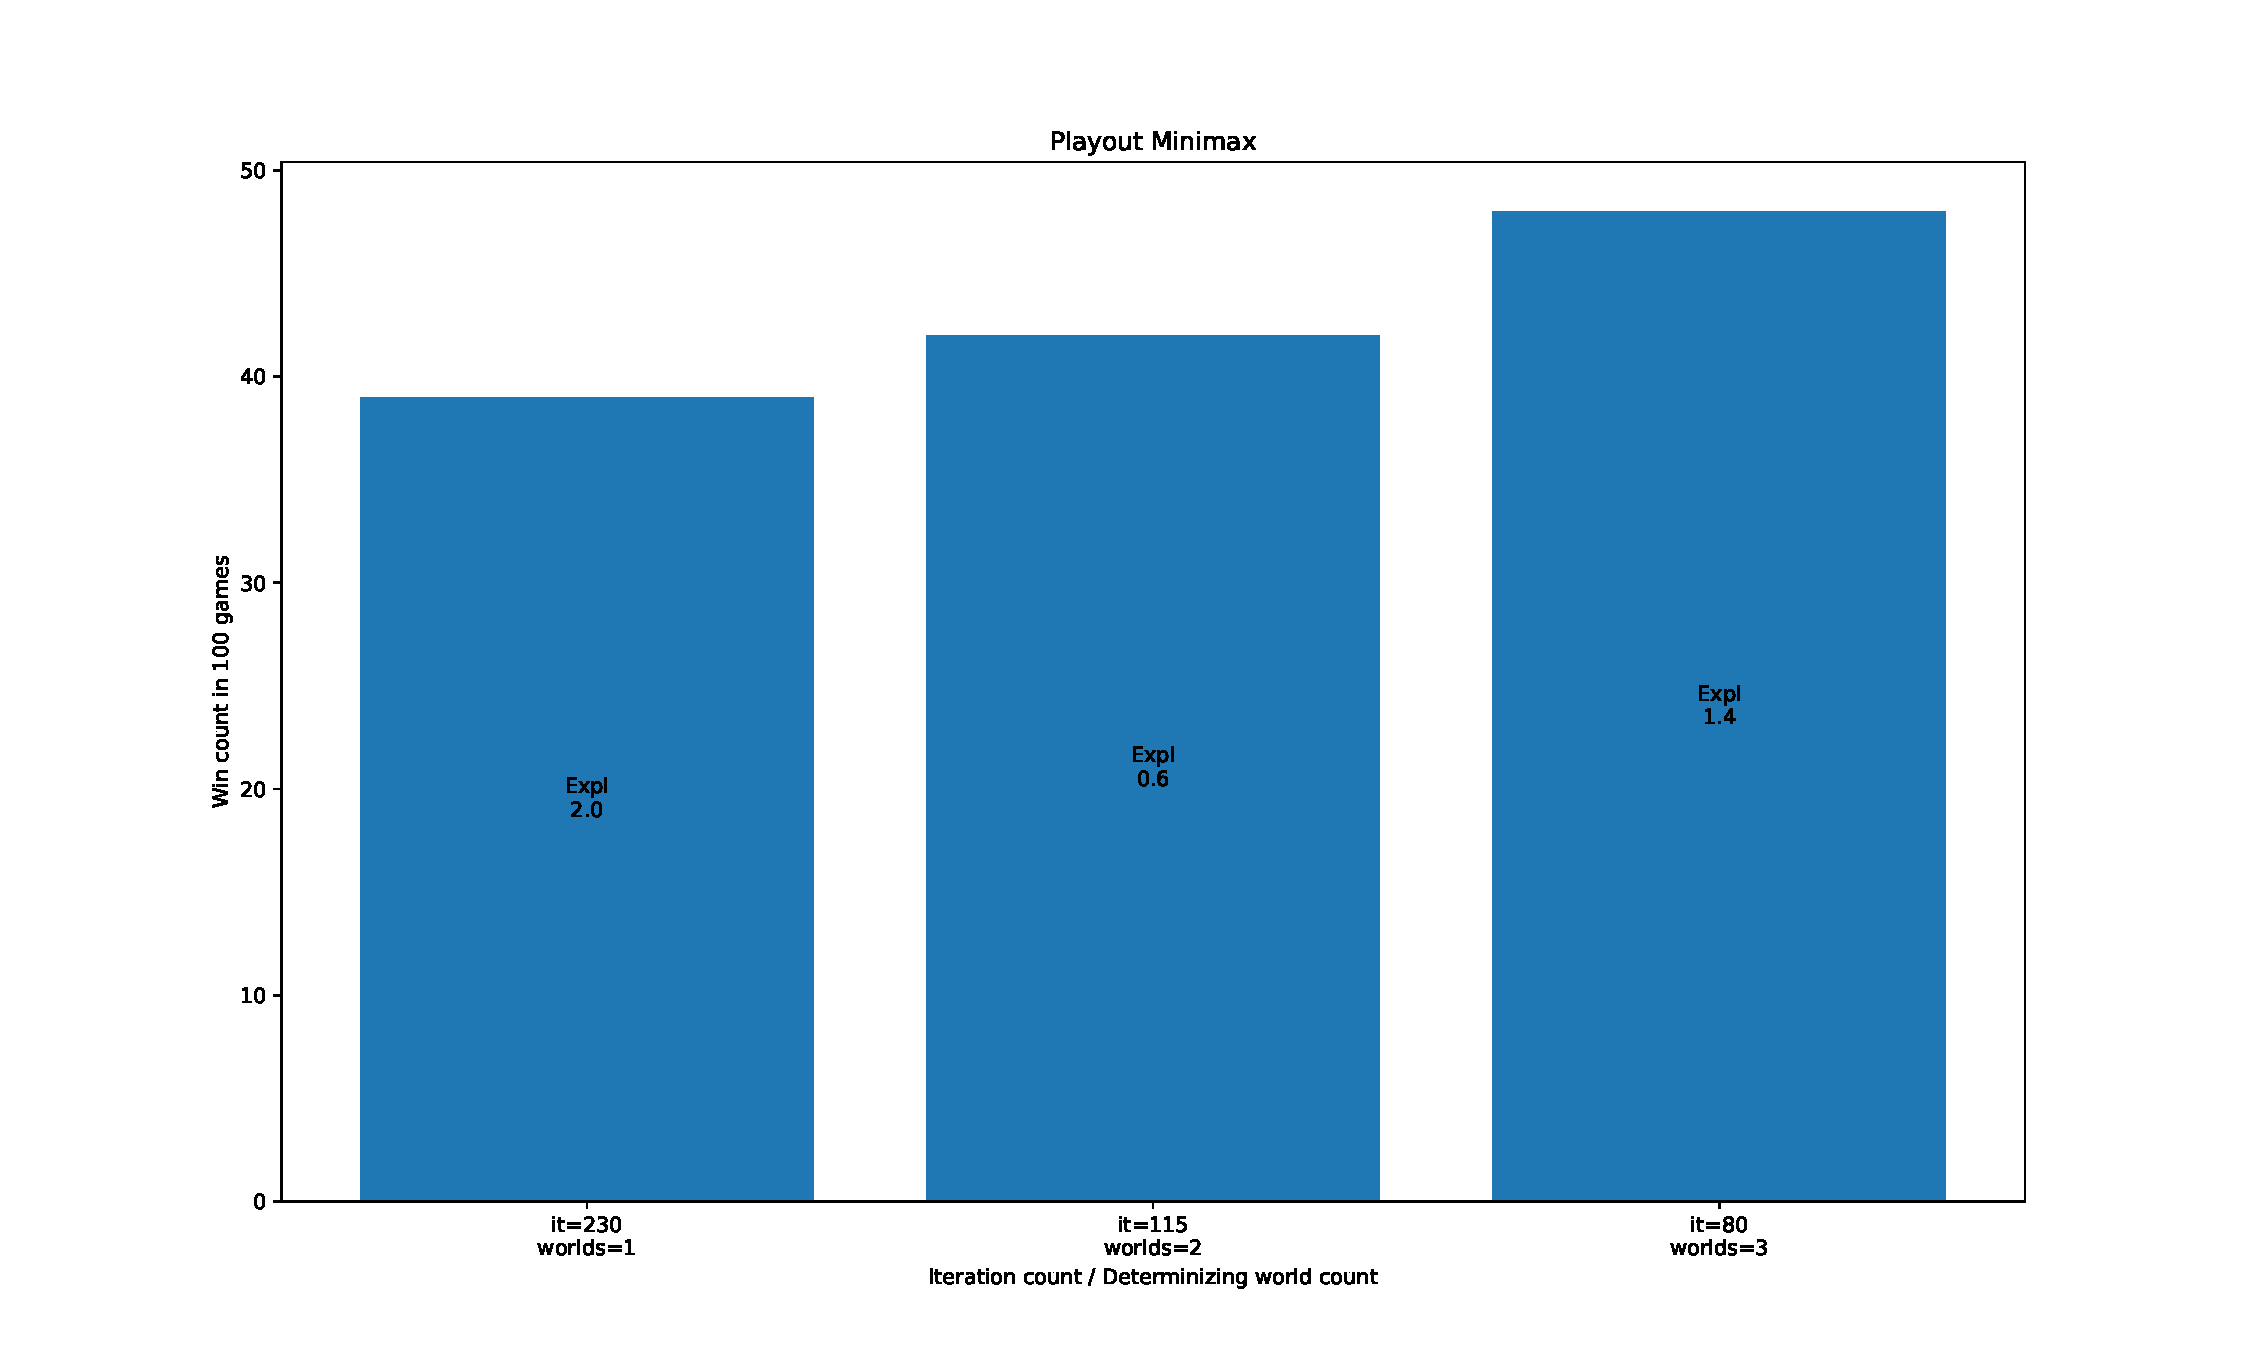
\includegraphics[width=170mm]{img/mcts_expl_worldcount_Minimax.pdf}}}
    \label{fig:example}
\end{figure}


\begin{figure}[H]
    \caption{Exploration constants producing the highest win rate in different iteration count-determinizing world count divisions for the Rules-based ALL MOVES playout}
    \centerline{\mbox{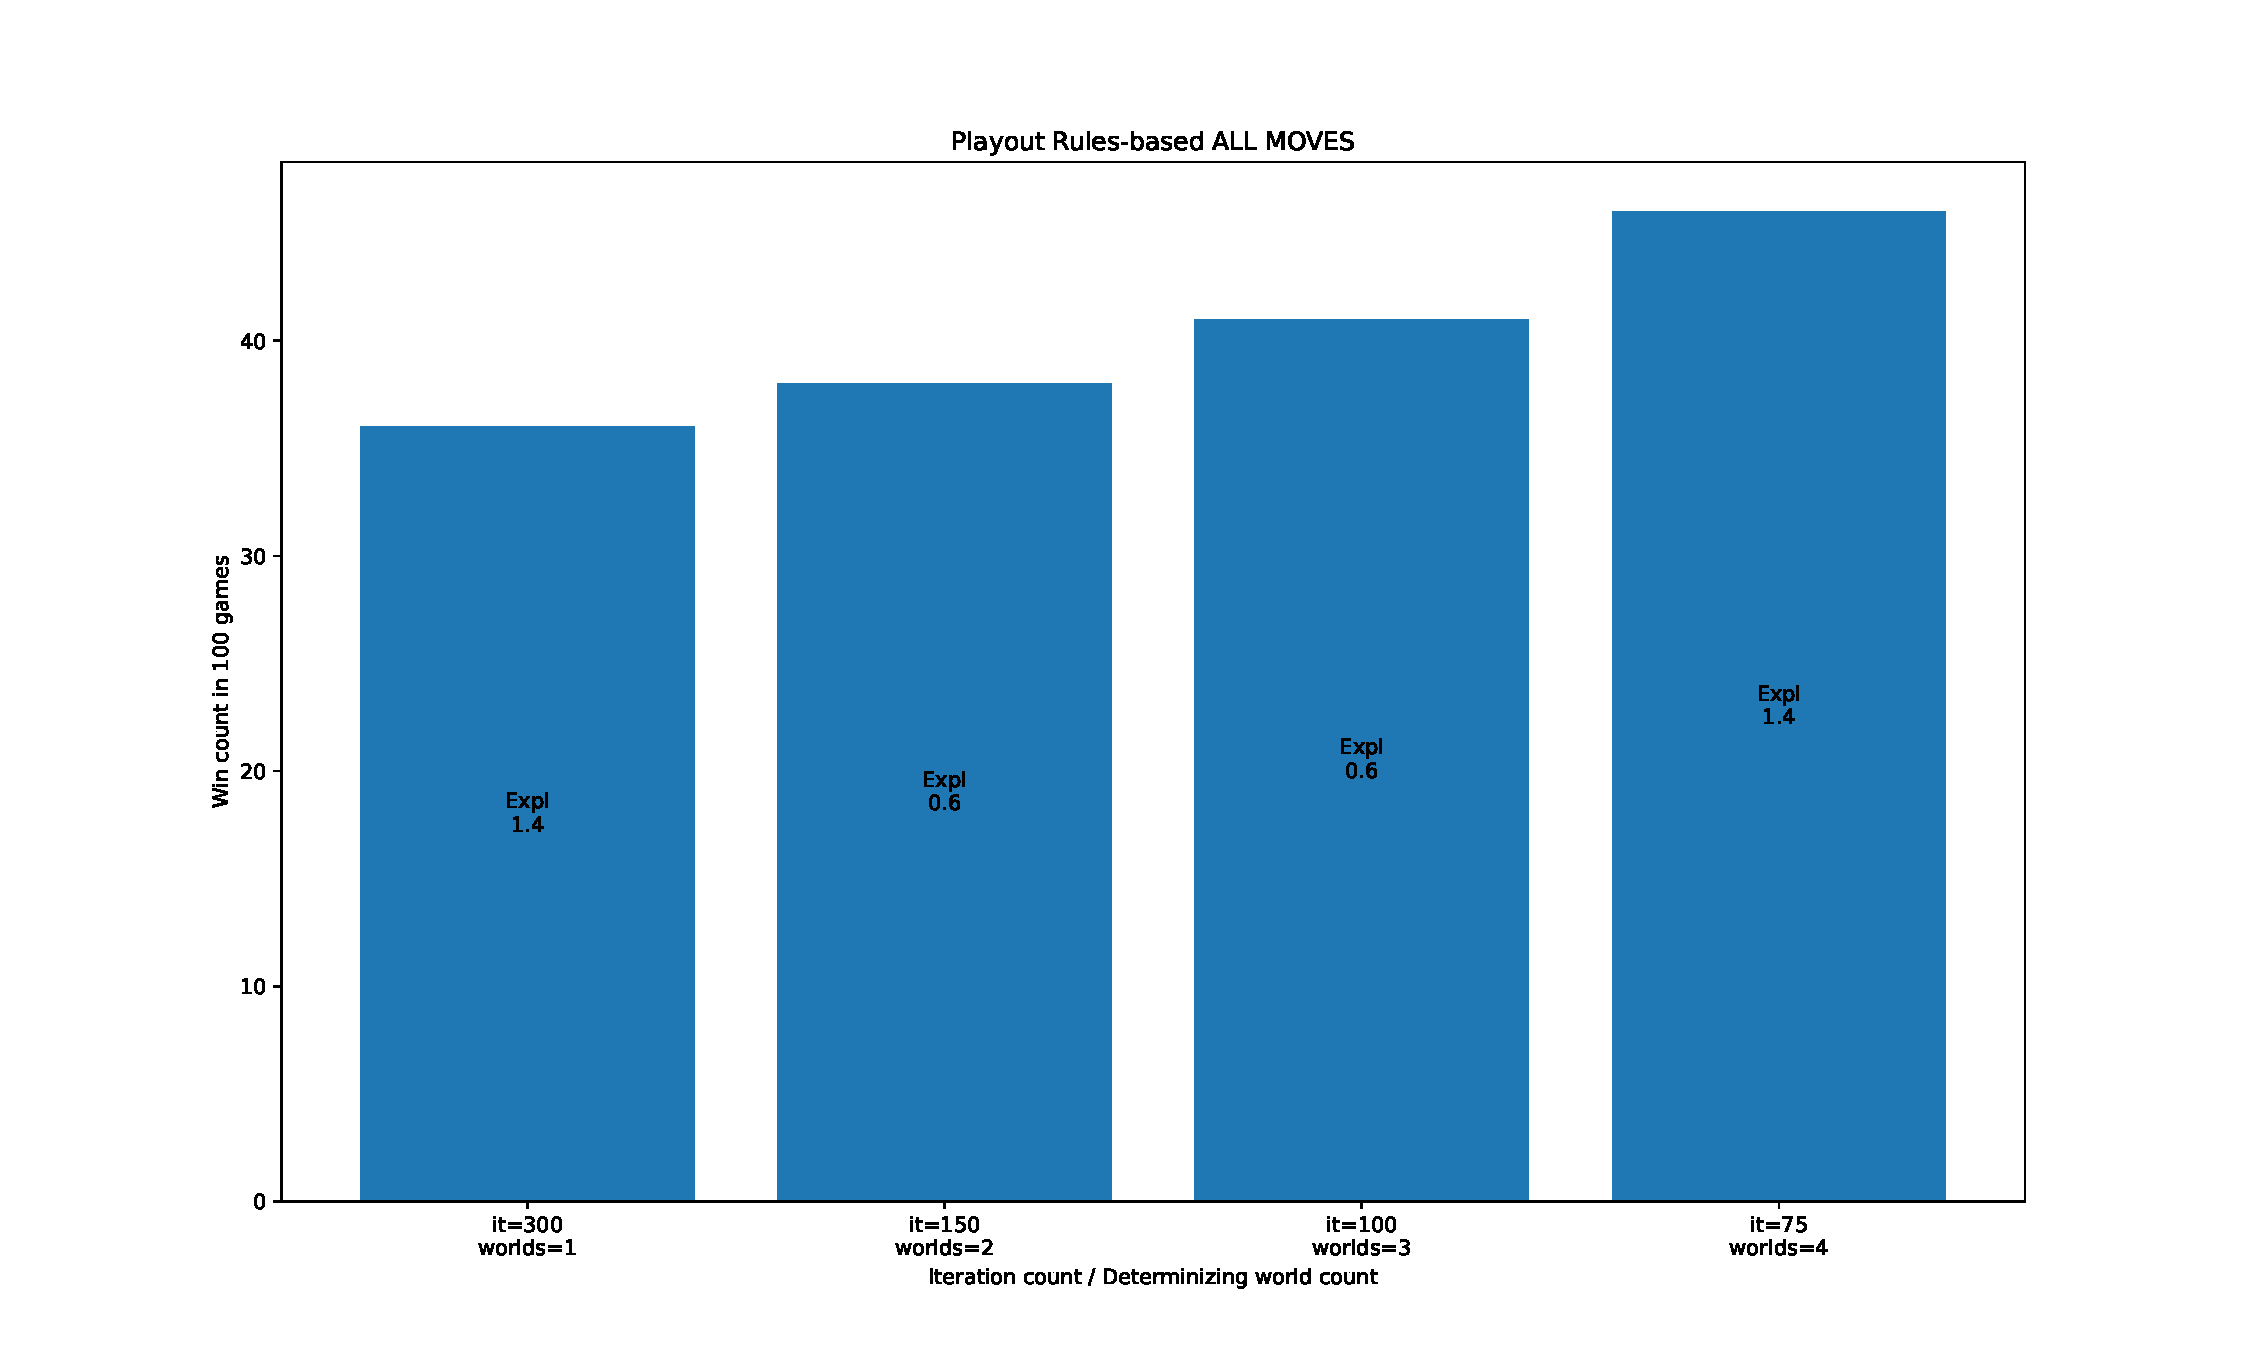
\includegraphics[width=170mm]{img/mcts_expl_worldcount_Rules-based ALL MOVES.pdf}}}
    \label{fig:example}
\end{figure}

\begin{figure}[H]
    \caption{Exploration constants producing the highest win rate in different iteration count-determinizing world count divisions for the Rules-based ONLY DTFM playout}
    \centerline{\mbox{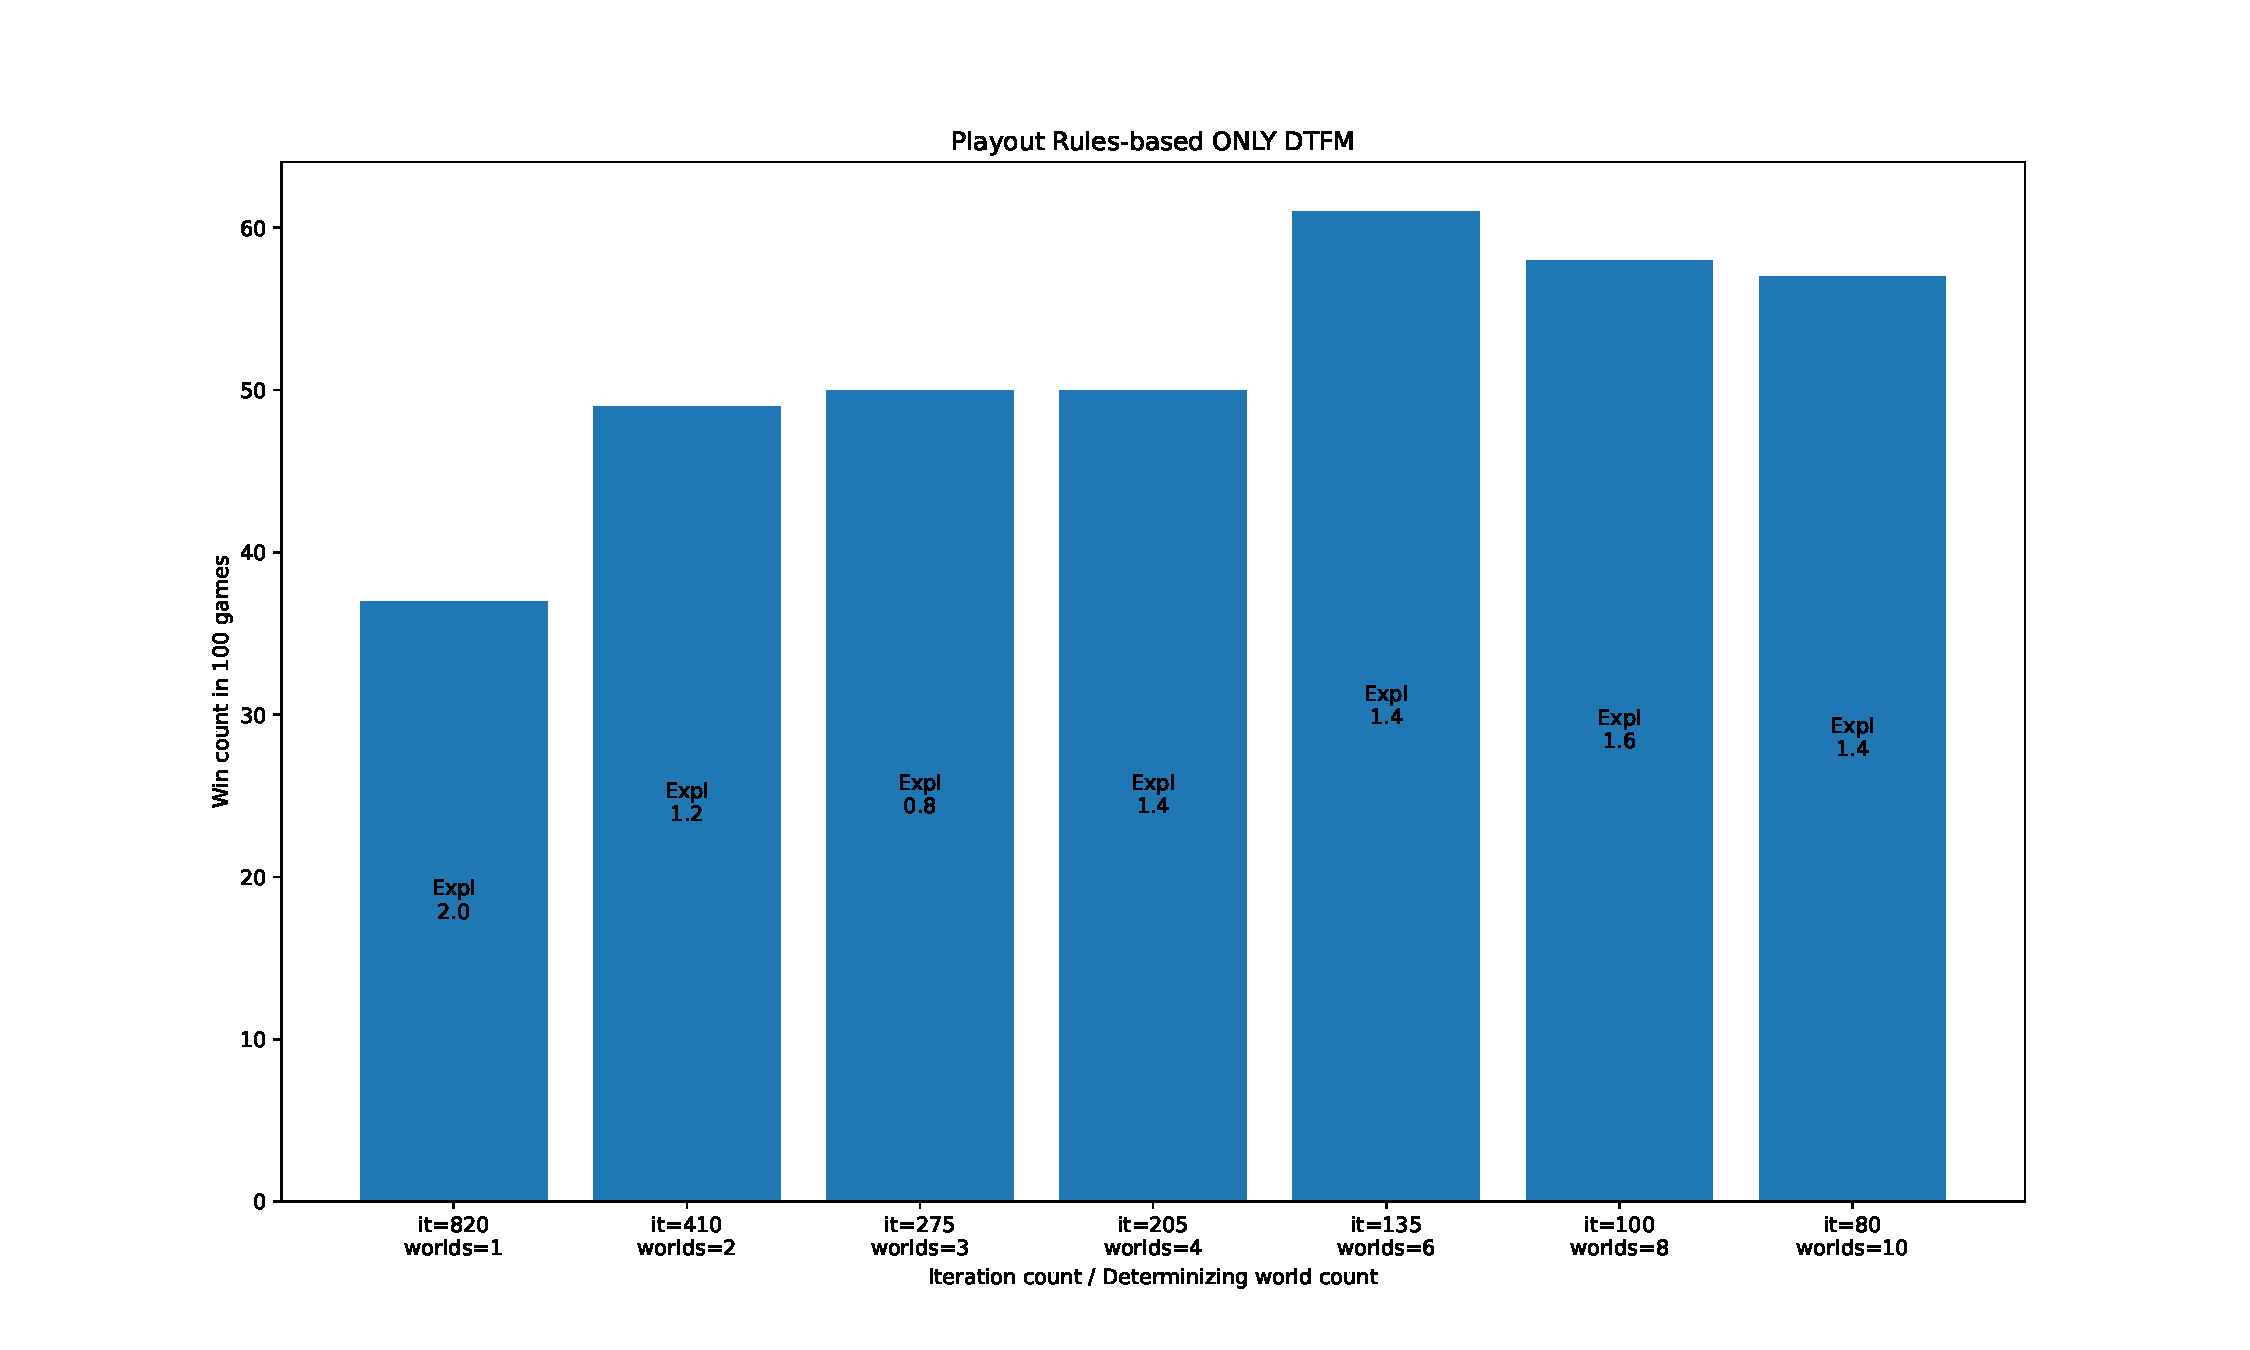
\includegraphics[width=180mm]{img/mcts_expl_worldcount_Rules-based ONLY DTFM.pdf}}}
    \label{fig:example}
\end{figure}

As seen in the second and third figures, the Minimax and the Rules-based ALL MOVES playout strategies don't achieve even 50\% of wins with any of the configured
exploration constants. For this reason, in the upcoming experiments, I will use following the configurations:


\begin{table}[H] 
    \centering
    \begin{tabular}{|c|c|c|} 
        \hline
        \textbf{Playout strategy} & \textbf{Iteration count} & \textbf{Exploration constant} \\ \hline
        First & 270 & 1.0 \\ \hline
        First & 360 & 1.8 \\ \hline
        Rules-based only dtfm & 135 & 1.4 \\ \hline
    \end{tabular}
    \caption{Strongest MCTS configurations against the Minimax-depth=3,worlds=1 agent}
    %\label{tab:example_table}
\end{table}


\section{Minimax}


\subsection{Hyperparameters} \label{subsec:Minimax_Hyperparameters}

Choosing the constants that represent the weights of the component weights in the HeuristicConstants structure is not a trivial task. After trying out different 
constants manually, I decided to automatize this task by creating random configurations, running some tournaments and evaluating the results. The two main attributes 
that could be maximized during this experiment are average points and win count. I chose to maximize average points because the experiment is run between
a minimax agent and one configured agent but the goal is to have the agent as strong as possible against all the other agents so choosing 
a configuration based on the win count against a concrete agent is the weaker option.


To obtain the current configuration, I ran an experiment of 10000 tournaments between the rules-based player and the minimax player. 
I chose to select the top 30 results i.e. the 30 tournaments that produced the highest average score for the minimax player. To achieve
this, I ran the following commands:

\begin{verbatim}
$ ./tournaments/minimax_random_config_experiment.py -v -e 10000  \ 
    -o heuristic_constant_experiments -p rules-based-strategy=only_dtfm 
$ ./tournaments/heuristic_const_experiment_evaluator.py -top 30 \
    -i tournament_results/heuristic_constant_experiments/ 
\end{verbatim}


and chose the configuration with the highest average score. This experiment produced the following weight constants:
\begin{table}[H] 
    \centering
    \begin{tabular}{|c|c|} % two centered columns
    \hline
    Weight constant name & Weight constant value \\ \hline
    OpponentInfluencingFactor & 9.83724229656198    \\ \hline
    PuocCompletablePower & 3.1133889400588606 \\ \hline
    MinusPointsPerUncompletableField & 373 \\ \hline
    CompletedPointsWeight & 416    \\ \hline
    MinusPointsPerUncompletablePuocPoints & 7  \\ \hline
    \end{tabular}
    \caption{Currently used heuristic weight constants}
    \label{tab:example_table}
\end{table}

Please notice that running this experiment with the current build will produce a different outcome since when I ran this experiment, I was using a previous build
and the old configuration for the minimax agent. The results of this experiment can be found in the \texttt{tournament\_results/heuristic\_constant\_experiments} directory.


\subsection{Search Depth and Determinizing World Count}

There are two other configurable parameters left after choosing the globally used heuristic weight constants as described in the previous section.
The goal of this section is to find the perfect balance between search depth and determinizing world count producing the strongest possible configuration.

The following table illustrates the determinizing world count for search depths fitting the time limit:

\begin{table}[H] 
    \centering
    \begin{tabular}{|c|c|}
        \hline 
        \textbf{Search depth} & \textbf{Determinizing world count} \\ \hline
        1 & 2000 \\ \hline
        2 & 200 \\ \hline
        3 & 20 \\ \hline
        4 & 2 \\ \hline
    \end{tabular}
    \caption{Minimax configurations fitting the time limit}
\end{table}




\section{Final Results}

In this section, I will present the final results of the players. This experiment employs a round-robin format meaning that every player plays against every other player.
First, a fixed number of 320 games were run in each tournament. To achieve the best results possible, additional tournaments of 160 games were run until a confidence interval
of 50\% was reached for any of the players. The upper bound for the number of games played between two concrete AI players was set to 2240. 
To eliminate any type of advantage, the tournaments were run with \texttt{the -b option} specified meaning that each seed is used twice, once with player1 as the initial player, 
and once with player2 as the initial player. This method helps to avoid any advantage connected with being the initial or the subsequent player. 

The following tables display the confidence interval and total games played between all other players and the minimax agents. Both tables have on the field in the i-th row
and j-th column the confidence interval of the j-th column's agent against the i-th row's agent. The following abbreviations for agent names are used in the following tables:
\begin{description}
    \item[Mini1,2000] - minimax-depth=1,worlds=2000
    \item[Mini2,200] - minimax-depth=2,worlds=200
    \item[Mini3,20] - minimax-depth=3,worlds=20
    \item[Mini4,2] - minimax-depth=4,worlds=2
    \item[MCTS135\_OD] - mcts-it=135,expl=1.4,worlds=6,playout=rules-based-strategy=only\_dtfm
    \item[MCTS270\_First] - mcts-it=270,expl=1.0,worlds=20,playout=first
    \item[MCTS360\_First] - mcts-it=360,expl=1.8,worlds=15,playout=first
    \item[RB\_OD] - rules-based-strategy=only\_dtfm
    \item[RB\_AM] - rules-based-strategy=all\_moves
\end{description}

\renewcommand{\arraystretch}{0.7} % Adjust the spacing between rows

\begin{table}[H] 
    \centering
    \begin{tabular}{|c|c|c|c|c|} 
        %\textbf{Search depth} & \textbf{Determinizing world count} \\ 
        \hline
        \text{ } & \textbf{Mini1,2000} & \textbf{Mini2,200} & \textbf{Mini3,20} & \textbf{Mini4,2} \\ \hline

        \multirow{2}{*}{\textbf{Mini1,2000}} & & 320 & 480 & 2240 \\
        & & 50.7\%-63.5\% & 52.0\%-62.4\% & 48.8\%-53.7\% \\ \hline
        \multirow{2}{*}{\textbf{Mini2,200}} & 320 & & 2240 & 2240 \\
        & 36.5\%-49.3\% & & 48.3\%-53.3\% & 47.5\%-52.5\% \\ \hline
        \multirow{2}{*}{\textbf{Mini3,20}} & 480 & 2240 & & 2240 \\
        & 37.6\%-48.0\% & 46.7\%-51.7\% & & 45.5\%-50.4\% \\ \hline
       \multirow{2}{*}{\textbf{Mini4,2}} & 2240 & 2240 & 2240 & \\
        & 46.3\%-51.2\% & 47.5\%-52.5\% & 49.6\%-54.5\% & \\ \hline

       \multirow{2}{*}{\textbf{MCTS135\_OD}} & 2240 & 2240 & 1280 & 1440 \\
        & 46.9\%-51.8\% & 48.7\%-53.6\% & 50.0\%-56.5\% & 50.3\%-56.4\% \\ \hline

       \multirow{2}{*}{\textbf{MCTS270\_First}} & 320 & 320 & 320 & 320 \\
        & 51.0\%-63.8\% & 51.0\%-63.8\% & 58.0\%-70.3\% & 58.6\%-70.9\% \\ \hline
       \multirow{2}{*}{\textbf{MCTS360\_First}} & 512 & 320 & 320 & 320 \\
        & 50.7\%-60.9\% & 55.7\%-68.2\% & 54.5\%-67.1\% & 56.0\%-68.5\% \\ \hline
       \multirow{2}{*}{\textbf{RB\_OD}} & 320 & 320 & 320 & 320 \\
        & 53.8\%-66.5\% & 60.8\%-73.0\% & 57.6\%-70.0\% & 57.0\%-69.4\% \\ \hline
       \multirow{2}{*}{\textbf{RB\_AM}} & 320 & 320 & 320 & 320 \\
        & 58.0\%-70.3\% & 63.7\%-75.6\% & 67.7\%-79.0\% & 62.5\%-74.4\% \\ \hline
       \multirow{2}{*}{\textbf{First}} & 320 & 320 & 320 & 320 \\
        & 94.5\%-98.9\% & 96.8\%-99.7\% & 93.7\%-98.5\% & 95.8\%-99.4\% \\ \hline
       \multirow{2}{*}{\textbf{Random}} & 320 & 320 & 320 & 320 \\
        & 97.2\%-99.9\% & 97.8\%-100.0\% & 97.2\%-99.9\% & 97.8\%-100.0\% \\ \hline
        
    \end{tabular}
    \caption{Minimax confidence intervals against all the other agents}
\end{table}

Looking at the last 4 rows of this table, it is clear that all the minimax agents easily won the tournaments against the First, Random
and the two strategies of the Rules-based agents. All these tournaments ended after the minimum amount of games were played that this experiment defines.
Deciding which minimax configuration is the strongest is not straightforward. The first 4 rows indicate that the 6 tournaments run between
the minimax agents against each other, 4 of the tournaments continued to the maximum number of games chosen for this experiment. The MCTS agents
with the First playout strategy produced weak results against all the minimax configurations. The single strong opponent was the MCTS agent
with the Rules-based only dtfm playouts. According to this experiment, the two strongest configurations were the one with a search depth of 3
and the one with the search depth of 4.

\begin{table}[H] 
    \centering
    \begin{tabular}{|c|c|c|c|} 
        %\textbf{Search depth} & \textbf{Determinizing world count} \\ 
        \hline
        \text{ } & \textbf{MCTS270\_First} & \textbf{MCTS360\_First} & \textbf{MCTS135\_OD} \\ \hline
        \multirow{2}{*}{\textbf{MCTS270\_First}} & & 2240 & 2240 \\
        & & 45.9\%-50.9\% & 48.1\%-53.0\% \\ \hline
        \multirow{2}{*}{\textbf{MCTS360\_First}} & 2240 & & 2240 \\
        & 49.1\%-54.1\% & & 48.2\%-53.1\% \\ \hline
        \multirow{2}{*}{\textbf{MCTS135\_OD}} & 2240 & 2240 & \\
        & 47.0\%-51.9\% & 46.9\%-51.8\% & \\ \hline
        \multirow{2}{*}{\textbf{Mini3,20}} & 320 & 320 & 1280 \\
        & 29.7\%-42.0\% & 32.9\%-45.5\% & 43.5\%-50.0\% \\ \hline
        \multirow{2}{*}{\textbf{Mini4,2}} & 320 & 320 & 1440 \\
        & 29.1\%-41.4\% & 31.5\%-44.0\% & 43.6\%-49.7\% \\ \hline
        \multirow{2}{*}{\textbf{Mini2,200}} & 320 & 320 & 2240 \\
        & 36.2\%-49.0\% & 31.8\%-44.3\% & 46.4\%-51.3\% \\ \hline
        \multirow{2}{*}{\textbf{Mini1,2000}} & 320 & 512 & 2240 \\
        & 36.2\%-49.0\% & 39.1\%-49.3\% & 48.2\%-53.1\% \\ \hline
        \multirow{2}{*}{\textbf{RB\_OD}} & 1280 & 1600 & 320 \\
        & 50.9\%-57.4\% & 50.5\%-56.3\% & 52.6\%-65.3\% \\ \hline
        \multirow{2}{*}{\textbf{RB\_AM}} & 320 & 480 & 320 \\
        & 55.1\%-67.6\% & 51.6\%-62.0\% & 62.5\%-74.4\% \\ \hline
        \multirow{2}{*}{\textbf{First}} & 320 & 320 & 320 \\
        & 92.9\%-98.0\% & 95.4\%-99.2\% & 96.8\%-99.7\% \\ \hline
        \multirow{2}{*}{\textbf{Random}} & 320 & 320 & 320 \\
        & 95.8\%-99.4\% & 96.3\%-99.6\% & 97.8\%-100.0\% \\ \hline
    
    \end{tabular}
    \caption{MCTS confidence intervals against all the other agents}
\end{table}

The last four rows show similar results as in the case of the minimax player meaning that the MCTS player is stronger than the 
First, Random and Rules-based agents. From the results of the tournaments run between the MCTS players, it is not possible
to choose the strongest configuration. Lastly, looking at the results against the minimax agent, the clear winner of the MCTS
configurations is the MCTS135\_OD.

\section{Deterministic vs Non-Deterministic World Results}

In this section, I will compare the results presented in the previous section with the same tournaments run in the deterministic world.
The same type of agents in the non-deterministic world are compared with the agents having the same computational resources in the 
deterministic world. This means that the minimax agent will use the same search depth and the MCTS player will use the same amount of iterations.

The main idea is to compare how imperfect information affects the different players. For this reason, I am comparing the following agents:

\begin{description}
    \item[minimax-depth=4]
    \item[mcts-it=820,expl=1.4,playout=rules-based-strategy=only\_dtfm]
    \item[mcts-it=5400,expl=1.0,playout=first]
    \item[mcts-it=5400,expl=1.8,playout=first]
\end{description}

Every tournament contained 320 games and the following table illustrates the results:

\begin{table}[H] 
    \centering
    \begin{tabular}{|c|c|c|c|c|} 
        \hline
        \textbf{Player name} & \textbf{Tournament wins} & \textbf{Confidence interval} \\ \hline
        MCTS820,expl=1.4,playout=only\_dtfm & 3 & 61.1\%-68.3\% \\ \hline
        Minimax4 & 2 & 45.9\%-53.4\% \\ \hline
        MCTS5400,expl=1.0,playout=first & 1 & 41.4\%-48.9\% \\ \hline
        MCTS5400,expl=1.4,playout=first & 0 & 36.8\%-44.1\% \\ \hline
    
    \end{tabular}
    \caption{Deterministic world results}
\end{table}

The MCTS player with the only\_dtfm playout strategy is clearly the strongest player in the deterministic world.